\clearpage
\section{Implementation details}
\subsection{Software design}
$DIYABC$ v2 has been designed in a very different way compared to version 1. Version 1 was a single executable file were the GUI \footnote{Graphic User Interface} and computation codes were highly intricated and both written in the same language (\emph{Delphi}). In version 2, the GUI and the computation codes have been completely separated. Actually, the GUI is a script written in \emph{python} and all computations are included in a program written in \emph{C++}. In opposition to \emph{Delphi} which is restricted to a single OS (\texttt{Windows}), \textit{python} and \textit{C++} can be used with the main three OS (\texttt{Linux}, \texttt{Mac} and \texttt{Windows}), allowing version 2  to be operated under all three OS.\\
The GUI uses the \textit{Qt} graphic library. The computation code is linked to the \textit{openmp} library allowing a better use of multicore/multiprocessor computers.\\
The GUI can launch the computation program with the right parameters and keeps track of the progress of the latter through small log files. The GUI can launch as many computation programs as there are open projects, but no more than one computation program per project. A \textit{lock} file located in the project directory is created when the computation program is launched by the GUI and removed when the computation program has normally terminated. When the computation program has exited anormaly, the GUI issues an error message trying to explain where the programm failed.    
\subsection{Files}
The program uses and produces various files which we will describe now.
\subsubsection{data files}
Data files are text files that contain information about the samples : number and names of microsatellite markers, multilocus genotypes of individuals. The basic  format is that of the Genepop software \citep{RR1995} and data files produced by DIYABC are under this format.  \textbf{Microsatellite genotypes must be noted with 3 (haploid) or 6 (diploid) digits, these three digit numbers being the length in nucleotides of the corresponding PCR products}. In addition, we have added some features to this basic format in order to use sequence data. All these additions are explained in section 4.4. SNP data correspond to a different file format, also detailed in section 4.4.\\ 
Any extension is accepted for datafile names, including no extension at all. If the data file is simulated with $DIYABC$, the extension is \texttt{mss} for microsatellite/DNA sequence data and \texttt{snp} for SNP data. The next page shows examples of data sets saved.

\subsubsection{reference table files} 
Reference table files are binary files which include two successive parts :
\begin{itemize}
 \item The first part is a header which contains information necessary to read the second part, such as the number of scenarios, or the number of parameters of each scenario.
 \item The second part contains simulated data set records, each record containing the scenario number, the parameter and summary statistics values.
\end{itemize}
 
 Each time a reference table is created or increased (each time the \fbox{\textsf{Run computation}} button is pressed), a text file is created in the project directory with the name \texttt{first\_records\_of\_the\_reference\_table\_X.txt} in which \texttt{X} is an integer number starting at 0 and increasing each time the \fbox{\textsf{Run computation}} button is pressed. This file provides a text version of the first $n$ newly created records of the reference table ($n$ being equal to the \emph{Particle loop size}, see section 3.7.3).\\

\subsubsection{output files}
As already seen, DIYABC achieves different analyses : comparison of scenarios, estimation of posterior distribution of parameters, model checking,  computation of bias and mean square errors and evaluation of confidence in scenario choice. Each analysis has its own output which can be printed and saved. Graphs are saved under the chosen format and non-graphic output are saved in text files.\\

We now describe all the files produced by each type of analysis. These files are located in directories (one directory per analysis) gathered in the \texttt{analysis} subdirectory of the project directory. Below is an example of the \texttt{TOYTEST2\_2012\_9\_26-1} project directory substructure:\\

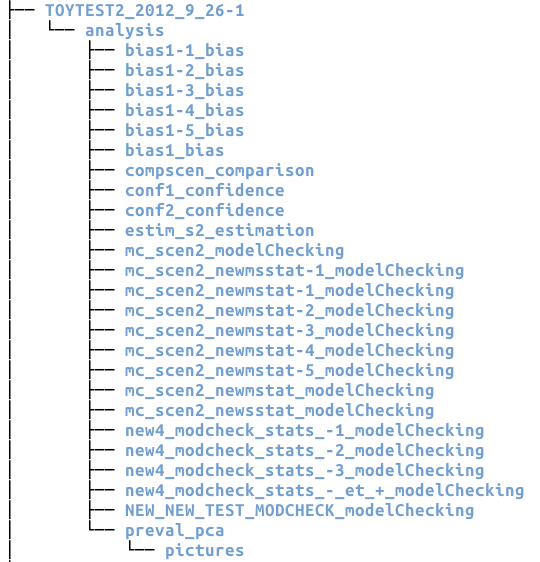
\includegraphics[scale=0.5]{gui_pictures/Capture-DIYABC-103.png}\\

Note that each directory name starts with the name of analysis followed by the type of analysis, $e.g.$ \texttt{bias} for a bias/precision analysis or \texttt{comparison} for a comparison of scenarios. In addition, when a picture has been saved, the corresponding file is located under a subdirectory named \texttt{pictures} ($e.g.$ at the bottom of the figure above).
\begin{description}
 \item [Pre-evaluate scenario prior combinations :] This analysis can produce two output files named \texttt{ACP.txt} and \texttt{locate.txt}. The former is the output of the Principal Component Analysis and the latter that of the analysis giving the proportion of simulated data sets which have a value below the observed value for every summary statistics. This latter file is exactly what appears in the GUI. The structure of the  \texttt{ACP.txt} file is the following. The first line indicates the number of points of the PCA, the number of PCA components (axes) and the inertia of each component, all values are separated by a single space. The second line provides the components of the observed data. It starts with a zero which corresponds to the scenario number in the following lines. Each subsequent line provides the components of data simulated according to a given scenario which number is at the beginning of the line. If one or more PCA figures have been saved, the corresponding files are saved in the \texttt{pictures} subdirectory. They are named as \texttt{refTable\_PCA\_X\_Y\_N.pdf}, with \texttt{X} and  \texttt{Y} giving the axis numbers and \texttt{N} being the number of represented points. 
 \item [Compute posterior probabilities of scenarios :] This analysis produces three output text files : \texttt{compdirect.txt}, \texttt{complogreg.txt} and \texttt{compdirlog.txt}. The latter is directly visualized in the GUI when clicking the \fbox{\textsf{view numerical results}} button. The first two files are used by the GUI to elaborate the two graphics (Direct approach and Logistic regression). Again, if graphics have been saved, the corresponding file(s) is(are) in the \texttt{pictures} subdirectory of the analysis directory.  
 \item [Evaluate confidence in scenario choice :] This analysis produces a single output file, \texttt{confidence.txt}, the content of which is visualized in the GUI.
 \item [Estimate posterior distributions of parameter :] Nine files are written as output of this type of analysis :
  \begin{itemize}
   \item three files \texttt{mmmq\_original.txt}, \texttt{mmmq\_composite.txt} and \texttt{mmmq\_scaled.txt} contain the statistics (mean, median, mode and quantiles) for the original, composite and scaled parameters, respectively. They are visualized in the GUI when clicking the \fbox{\textsf{view numerical results}} button. 
   \item three files \texttt{paramstatdens\_original.txt}, \texttt{paramstatdens\_composite.txt} and \texttt{paramstatdens\_scaled.txt} are used by the GUI to produce the graphics showing prior/posterior distribution.
   \item three files \texttt{phistar\_original.txt}, \texttt{phistar\_composite.txt} and \texttt{phistar\_scaled.txt} contains the $\phi^*$ values of the original, composite and scaled parameters, respectively. These files can be used for instance to redraw posterior distributions, $e.g.$ with the $R$ software.
  \end{itemize}
As already mentionned, saved graphics are located in a \texttt{pictures} subdirectory.
 \item [Compute bias and precision of parameter estimations :] Three files \texttt{bias\_original.txt}, \texttt{bias\_composite.txt} and \texttt{bias\_scaled.txt} are produced by this type of analysis. All three files are visualized in the GUI. 
 \item [Perform model-checking] The output files of this type of analysis are the same as those of the \textit{Pre-evaluate scenario prior combinations} analysis (see above). The only difference is in the names of the two text files which start with \texttt{mc} for \texttt{model checking}. 
\end{description}
~\\

In addition, the GUI program writes several files in the project directory :
\begin{description}
 \item [command.txt :] this text file contains the history of commands issued by the GUI to be achieved by the computation program.
 \item [conf.analysis :] this text file contains information about analyses.
 \item [conf.gen.tmp :] this text file contains information about the loci, the genetic parameters and the summary statistics.
 \item [conf.hist.tmp :] this text file contains information about the scenario and the historical parameters.
 \item [conf.th.tmp :] This text file contains the title line of the reference table.
 \item [conf.tmp :] This text file contains the name of the dataset and the number of parameters and summary statistics.
 \item [header.txt :] This text file is a concatenation of the previous four files and is red by the computation program.
 \item [xxx.diyabcproject :] This text file contains the path to the \texttt{xxx} project.
 \item [RNG\_state\_0000.bin :] This binary file contains the current state of the random generator.
 \item [init\_rng.out :] This text file contains information about the initialization of the random generator.
\end{description}
~\\

The computation program writes the following files in the project directory :
\begin{description}
 \item [reftable.log :] This text file is produced when a reftable is increased. It provides the GUI with information about the progress of computations : achieved number of records, time left.
 \item [statobs.txt :] This text file is written every time an analysis is performed. It contains the values of summary statistrics for the observed data set.
\end{description}

The following files are output by the computation program everytime it has been launched by a specific command of the GUI (their use is only for debugging purposes and they are all in the project directory) :
\begin{description}
 \item [general.out :] when computing a reftable.
 \item [pre-ev.out :] when performing a \textit{Pre-evaluate scenario prior combinations} analysis.
 \item [compare.out :] when performing a \textit{Compare scenarios} analysis.
 \item [confidence.out :] when performing a \textit{Confidence in scenario choice} analysis.
 \item [estimate.out :] when performing a \textit{ABC parameter estimation} analysis.
 \item [bias.out :] when performing a \textit{bias-precision} analysis.
 \item [modelChecking.out :] when performing a \textit{model checking} analysis.
\end{description}

When performing a \textit{Bias-precision} or a \textit{Confidence in scenario choice} analysis, the computation program simulates what we call \textit{pseudo-observed datasets}. The parameter and summary statistics values of these pseudo-observed datasets are written in a text file named \textbf{pseudo-observed\_datasets\_xxx.txt} in which \textbf{xxx} is the name given to the analysis.


\subsection{Missing data}
Missing or undetermined genotypes should be coded as \texttt{000} (haploid microsatellites), \texttt{000000}  (diploid microsatellites), \texttt{$<[~]>$} (haploid sequences) or \texttt{$<[~][~]>$} (diploid sequences) and \texttt{9} (SNP) in the data file. \\
Missing data are taken into account in the following way. For each appearance of a missing genotype in the observed data set, the programs records the individual and the locus. When simulating data sets, the program replaces the simulated genotype (obtained through the coalescence process algorithm) by the missing data code at all corresponding locations. All summary statistics are thus computed with the same missing data as for the observed data set. 

\subsection{Data files}
There are two different incompatible formats for data files, one for SNP loci and the other for microsatellite/DNA sequence data.\\ For the microsatellite/DNA sequence data, the format already presented in version 1 of DIYABC is an extended Genepop format. The additional features are :
\begin{enumerate}
\item In the title line appears the sex ratio noted between \textsf{$<$} and \textsf{$>$} under the form \textsf{$<NM=rNF>$}, in which $r$ is the ratio of the number of females per male ($e.g.$ \textsf{$<NM=2.5NF>$} means that the number of males is 2.5 times the number of females). Since the title is generally only copied, this addition should not interfere with other programs using  Genepop datafiles. Also if there is no such sex ratio addition, DIYABC will consider by default that NM=NF.
\item After the locus name, there is an indication for the category of the locus which is $<A>$ for autosomal diploid loci, $<H>$ for autosomal haploid loci, $<X>$ for X-linked (or haplo-diploid) loci, $<Y>$ for Y-linked loci and $<M>$ for mitochondrial loci. If no category is noted, DIYABC will consider the locus as autosomal diploid or autosomal haploid depending on the corresponding genotype of the first typed individual.
\item Genotypes of microsatellite loci are noted with six digit numbers (e.g. 190188) if diploid and by three digit numbers (e.g. 190) if haploid.
\item Sequence locus are noted between  \textsf{$<$} and \textsf{$>$} . In addition each sequence allele is noted between brackets. For instance, a haploid sequence locus  will be noted $<[$GTCTA$]>$ and a diploid sequence locus $<[$GTCTA$][$GTCTT$]>$.
\item Missing microsatellite genotypes are noted \textsf{000} if haploid or \textsf{000000} if diploid.
\item Missing sequence genotypes are noted $<[\ ]>$ if haploid or $<[\ ][\ ]>$ if diploid.
\end{enumerate}

For SNP data, the format includes:
\begin{itemize}
 \item a first line providing the sex-ratio as above and any text that can be used as a title (the sex ratio can be anywhere in this line).
 \item a second line starting with the three keywords \texttt{IND  SEX  POP}, separated by at least one space, followed by as many letters as SNP loci, the letter giving the location of the locus as above ($<A>$ for autosomal diploid loci, $<H>$ for autosomal haploid loci, $<X>$ for X-linked (or haplo-diploid) loci, $<Y>$ for Y-linked loci and $<M>$ for mitochondrial loci). Letters are separated by a single space.
 \item as many lines as there are genotyped individuals, with the code-name of the individual, a letter ($M$ or $F$) indicating its sex, a code-name for its population and the values (0, 1 or 2) of the number of the (arbitrarily chosen) reference allele at each SNP locus. 0 = homozygous genotype for the non reference allele, 1 = heterozygous genotype for the reference allele, 2 = homozygous genotype for the reference allele.
\end{itemize}


 
Below are three examples of data sets that can be analyzed with DIYABC.\\ In the first example, this data set includes two population samples, each of 12 diploid individuals (8 females and 4 males in the first sample and 5 females and 7 males in the second sample). As deduced from the letter between $<$ and $>$ on the locus name lines (see page 25), these individuals have been genotyped at 3 microsatellite loci (1 autosomal $<A>$, 1 X-linked $<X>$ and 1 Y-linked $<Y>$) and 3 DNA sequence loci (1 autosomal. 1 X-linked and 1 mitochondrial $<M>$). The species sex-ratio, given in the title line, is of three males for one female ($<NM=3NF>$) or in other words, the number of males equals three times the number of females. 
\begin{figure}[h]
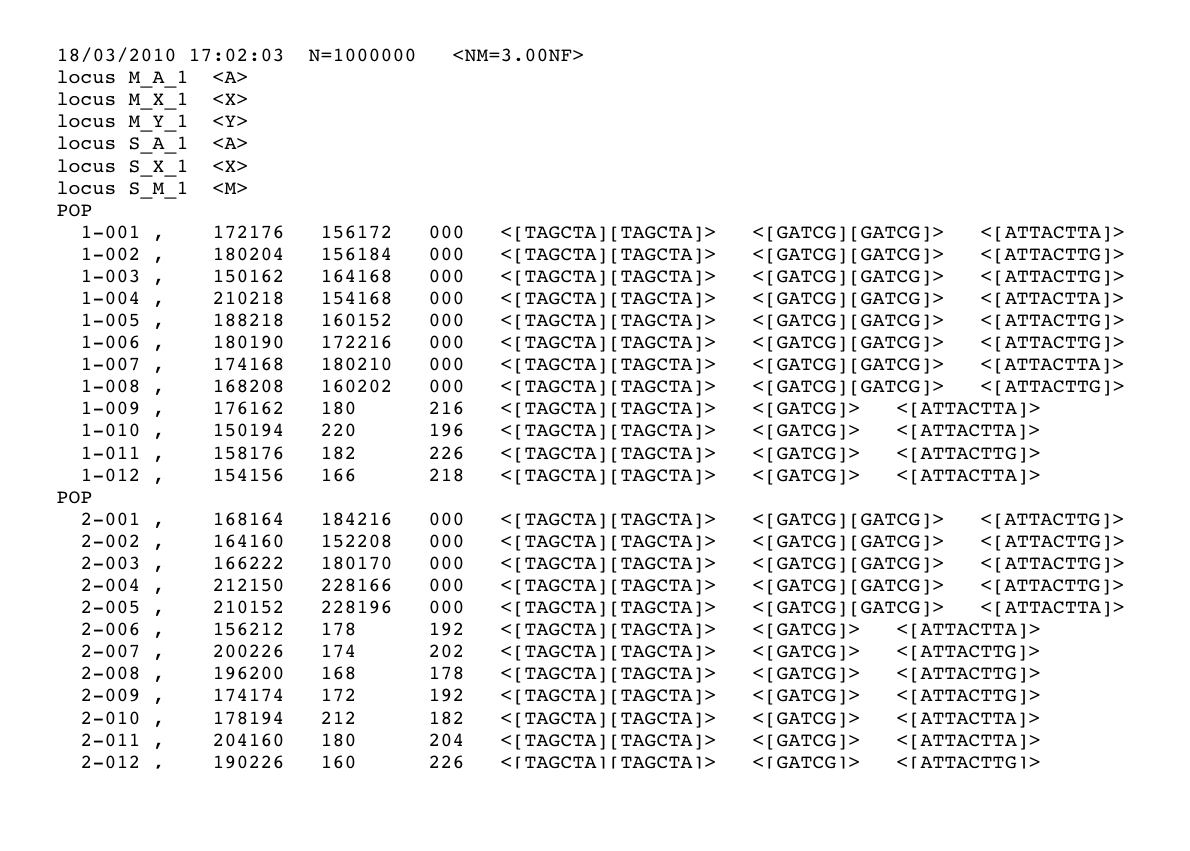
\includegraphics[scale=0.6]{gui_pictures/screenga001.png}
\end{figure}
\newpage
In the second example, the species is haploid. Individuals have been genotyped at three autosomal microsatellite loci and one mitochondrial DNA sequence locus. The species being haploid (deduced from the presence of autosomal haploid loci), no indication of the sex-ratio appears in the title line.

\begin{figure}[h]
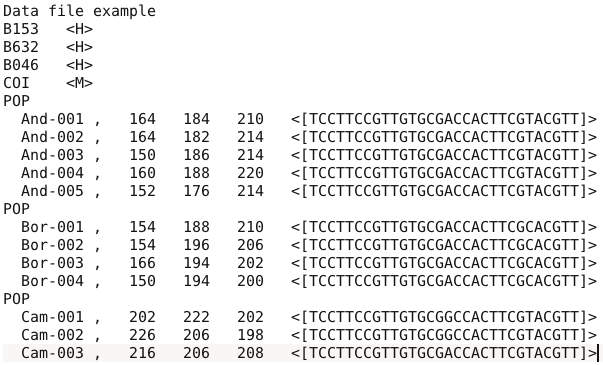
\includegraphics[scale=0.6]{gui_pictures/screenga002.png}
\end{figure}

In the third example, the species is diploid and has been genotyped at a large number of SNP autosomal loci. The first line provides the title which includes the species sex-ratio. The second line indicates what's in the different columns : individual name in column 1, individual sex in column 2, population name in column 3 and one column per SNP locus (the letter \texttt{A} indicates that the autosomal locus is autosomal; it would be \texttt{X} for an X-linked locus, \texttt{Y} for a Y-linked locus and \texttt{M} for a mitochondrial locus) . Columns are sparated by one or more spaces. SNP are coded 0, 1 or 2 according to the number of reference alleles at the corresponding locus. Only the top left part of the data file is represented below :

\begin{figure}[h]
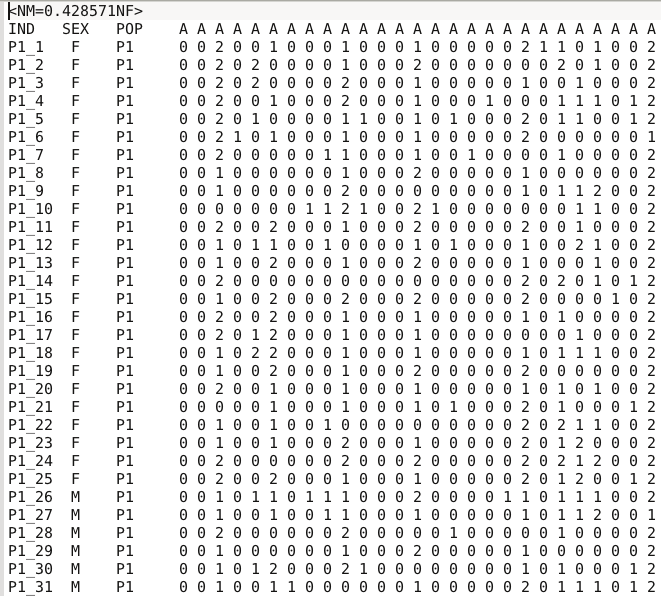
\includegraphics[scale=0.5]{gui_pictures/screenga003.png}
\end{figure}



\clearpage
\section{Cluster version}\label{cluster}
The ABC method requires simulating many data sets, which is time consuming. Typically, one to several millions data sets are needed to build up an interresting reference table and this process can last several hours to several days. Hence it might be useful to take advantage of a computer grid cluster.

This part of the notice describe how to use a cluster with the GUI frontend in Section~\ref{sub:proceed}. Advices to distribute the workload in jobs on the cluster are given in Section~\ref{sub:advices}. For advanced users who need more information, Section~\ref{sub:node.sh} describes the jobs that are sent to the queueing system of the cluster, and Section~\ref{rng} sums up how DIYABC produces independent random number generators (RNG's).

\subsection{Using a cluster with DIYABC}\label{sub:proceed}
You can prevent DIYABC from simulating data sets on your own computer by checking \textsf{use a cluster} in the setting panel of the GUI. Then, instead of computing the simulations on your computer, the GUI frontend will prepare a bundle for the cluster. Note that, while this option remains checked, DIYABC will not compute any reftable on your computer. 
\\
Generating a reference table with a cluster is a three stage process.
\begin{description}%\setlength{\itemsep}{0pt} \setlength{\topsep}{0pt} \setlength{\partopsep}{0pt} \setlength{\parsep}{0pt}  \setlength{\parskip}{0pt}%
 \item[1st stage] Configure the required parameters in the GUI frontend and generate the cluster bundle (set of zipped files).
 \item[2nd stage] Transfer the bundle to the cluster and run it.
 \item[3rd stage] Transfer back the reference table and include it to the project
\end{description}

%\subsubsection{Configure the required parameters in the GUI frontend and generate the cluster bundle}\label{clusterconfigure}
In the cluster tab of the settings panel, you can configure the useful parameters to send correct orders to the job scheduler of your cluster. The bash script named \texttt{launch.sh} of the cluster bundle produced by the GUI will sent those orders to the job scheduler of the cluster. To be able to write this bash script, the GUI needs informations on our cluster you can give by filling the fields of the cluster tab. \\

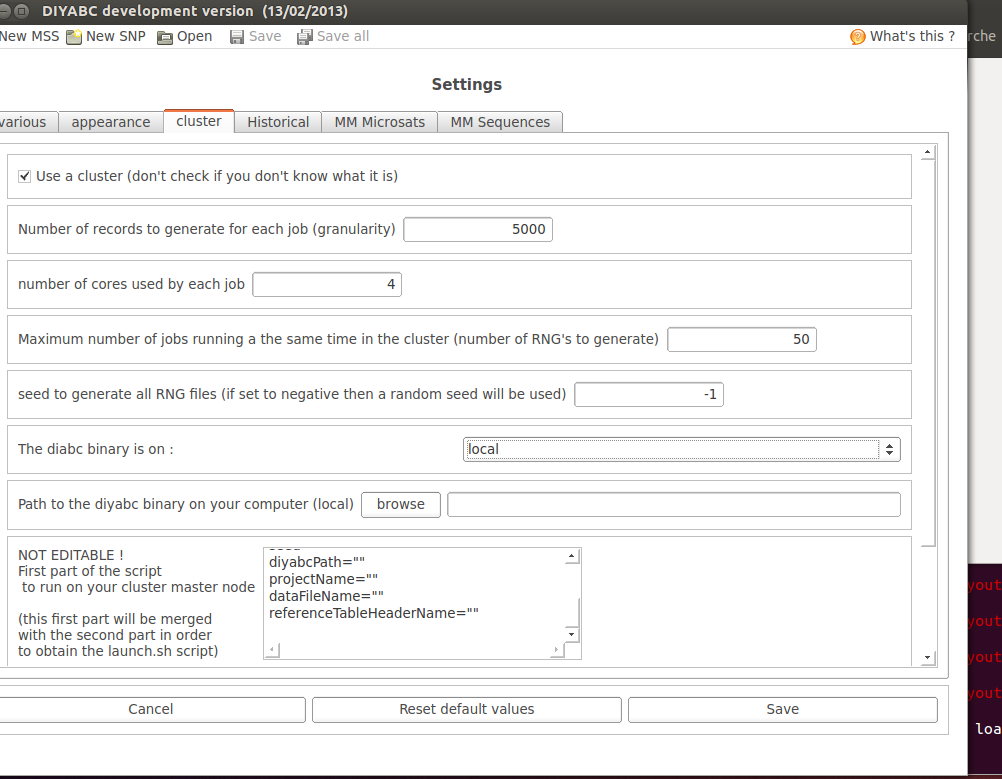
\includegraphics[scale=0.33]{gui_pictures/Capture-DIYABC-cluster.png} \\

\subsubsection{Configuring distribution of the workload on the cluster}

You have to understand and edit six parameters of the cluster settings. We shall recall here that the ``diyabc binary'' program is able to take advantage of multi-core computers. Thus to divde the whole workload, the cluster bundle can run several jobs, and configure each job to use several CPU cores of a given machine in the cluster\footnote{The multi-threaded capacity of DIYABC was programmed with the OpenMP API. This means that DIYABC can use several cores in a single computer but, contrary to MPI-based program, a single job cannot use several cores distributed on different computers. So please be sure to use an apropriate parallele environment to submit your jobs. Ask to your cluster system administrator.}. 
The six parameters might be given by filling the blank fields of the cluster tab, and are as follow.
\begin{itemize}\setlength{\itemsep}{0pt} \setlength{\topsep}{0pt} \setlength{\partopsep}{0pt} \setlength{\parsep}{0pt}  \setlength{\parskip}{0pt}%
\item ``\textit{Number of simulations oer job (granularity)}'' or \texttt{numSimulatedDatasetByJob}: This integer indicates the number of data sets simulated by each single job. It represents the granularity of your computations on the cluster.
\item ``\textit{Number of cores per job}'' or \texttt{coresPerJob}: This integer indicates how many CPU cores will be used by each job.
\item ``\textit{Maximum number of jobs running at the same time in the cluster}'' or \texttt{maxConcurrentJobs}: This integer indicates the maximum number of jobs allowed to run simultaneously on the cluster.
\item ``\textit{First seeds of the RNG's}'' or \texttt{seed}: This integer indicates to DIYABC the seeds to initialize the RNG's. By writing \texttt{-1} you ask the program to use random seeds (recommended). Starting from user-defined seeds is mainly for testing or debbugging purposes. 
\item ``\textit{The diyabc binary is on}'': This option determines whether the diyabc binary program (\texttt{general}) is already installed on the cluster (then set \texttt{cluster}) or if the bundle has to import a suitable binary (then set \texttt{local}).
\item ``\textit{Path to the diyabc binary}'' or \texttt{diyabcPath}: This string indicates the path of a diyabc binary program that can run on the machines of the cluster. Note that the binary can be on your own computer (you can browse your file system to choose the correct diyabc binary with the dedicated button) or on your cluster, in which case it is highly recommanded to specify an absolute path. 
\end{itemize}



\subsubsection{Dealing with the job scheduler of the cluster}


The two last text boxes of the cluster tab in the settings panel deal with the main script \texttt{launch.sh} executed on the master node of the cluster. This script  generates a pool of RNG files, submits the jobs to the scheduler queuing system using a \texttt{node.sh} script, monitors the jobs and merges all reftable files into a single reftable file when all jobs are completed.
The last box (which is the only one that be edited) deals with the jobs submission. By default, \texttt{launch.sh} targets a \textit{Grid Engine} cluster. You probably need to customise this script to fit your cluster configuration (scheduler system, queue name, ...). You should mainly need to modify the  \texttt{\#\#\#\#\# EDIT \#\#\#\#\#} section to comply with the rules of the job queueing system of the cluster. Please ask for help to your cluster system administrator.


\subsubsection{Transfer the bundle to the cluster and run it}\label{clusterrun}
Once you have checked the box \textsf{Use a cluster (...)}, configured the cluster parameters in the settings panel and saved them, you need to click on the \fbox{\textsf{Run computation}} button from your project panel. The program will ask you the name of the tar archive you will have to copy on the cluster to run the computations. This tar archive can be copied to your cluster account by many ways (for instance with the help an sftp client like FileZilla or WinSCP). Once the archive is on your cluster working directory, you can log in your cluster account with a shell console and untar your archive by typing :\\
%\fbox{
   \begin{minipage}{0.9\textwidth}
\begin{lstlisting}
tar -xvf <yourTarArchiveName.tar>
cd yourTarArchiveName
\end{lstlisting}
   \end{minipage}\\
%}

 This will create a directory with all the files needed to run DIYABC, namely
\begin{enumerate}
    \item \textsf{general} : the DIYABC binary program or executable
    \item \textsf{header.txt} : the header file
    \item \textsf{launch.sh} : the main script to run
    \item \textsf{node.sh} : the script that will be runned by your scheduler for each job
    \item \textsf{$<yourData.mss>$} : the data file 
\end{enumerate}
You can now run the main script by typing \texttt{./launch.sh} in the
shell console. If everything was set correctly, you can monitor the progression of the computations in the console. For instance, for a total of 50,000 data sets to be produced through 5 jobs of 10,000 data sets:\\
%\fbox{%
   \begin{minipage}{0.99\textwidth}
 
\definecolor{dkgreen}{rgb}{0,0.6,0}
\definecolor{gray}{rgb}{0.5,0.5,0.5}
\definecolor{mauve}{rgb}{0.58,0,0.82}
 
\lstset{ 
  language=bash,                % the language of the code
  basicstyle=\footnotesize,           % the size of the fonts that are used for the code
  numbers=left,                   % where to put the line-numbers
  numberstyle=\tiny\color{gray},  % the style that is used for the line-numbers
  stepnumber=1,                   % the step between two line-numbers. If it's 1, each line 
                                  % will be numbered
  numbersep=5pt,                  % how far the line-numbers are from the code
  backgroundcolor=\color{white},      % choose the background color. You must add \usepackage{color}
  showspaces=false,               % show spaces adding particular underscores
  showstringspaces=false,         % underline spaces within strings
  showtabs=false,                 % show tabs within strings adding particular underscores
  frame=single,                   % adds a frame around the code
  rulecolor=\color{black},        % if not set, the frame-color may be changed on line-breaks within not-black text (e.g. comments (green here))
  tabsize=4,                      % sets default tabsize to 2 spaces
  captionpos=b,                   % sets the caption-position to bottom
  breaklines=true,                % sets automatic line breaking
  breakatwhitespace=false,        % sets if automatic breaks should only happen at whitespace
  title=\lstname,                   % show the filename of files included with \lstinputlisting;
                                  % also try caption instead of title
  keywordstyle=\color{black},          % keyword style
  commentstyle=\color{dkgreen},       % comment style
  stringstyle=\color{mauve},         % string literal style
  escapeinside={\%*}{*)},            % if you want to add LaTeX within your code
  morekeywords={*},              % if you want to add more keywords to the set
  deletekeywords={}              % if you want to delete keywords from the given language
}


\begin{lstlisting}
>launch.sh
** Generation of RNG files :
./general -p ./ -n "t:1;c:5;s:1038"

** jobs submition :

qsub -N n1_test -q short.q -cwd node.sh 10000 /home/dehneg/DIYABCtest 1  test.mss
Your job 111598 ("n1_test") has been submitted

qsub -N n2_test -q short.q -cwd node.sh 10000 /home/dehneg/DIYABCtest 2  test.mss
Your job 111599 ("n2_test") has been submitted

qsub -N n3_test -q short.q -cwd node.sh 10000 /home/dehneg/DIYABCtest 3  test.mss
Your job 111600 ("n3_test") has been submitted

qsub -N n4_test -q short.q -cwd node.sh 10000 /home/dehneg/DIYABCtest 4  test.mss
Your job 111601 ("n4_test") has been submitted

qsub -N n5_test -q short.q -cwd node.sh 10000 /home/dehneg/DIYABCtest 5  test.mss
Your job 111602 ("n5_test") has been submitted

** monitoring :
0/5 finished 0%  (total : 0)
1/5 finished 20% (total : 10000)
1/5 finished 20% (total : 10000)
2/5 finished 40% (total : 20000)
4/5 finished 80% (total : 40000)
5/5 finished 100% (total : 50000)

** reftables concatenation  :
./general -p /home/dehneg/DIYABCtest -q 2>&1 concat.out
*************************************************************
All the result files have been concatenated into reftable.bin
See concat.out output file for logs
*************************************************************
\end{lstlisting}
   \end{minipage}\\

%}
% \begin{enumerate}
%     \item line 3 : generation of all RNG files : \textsf{RNG\_state\_0000.bin}, ..., \textsf{RNG\_state\_0005.bin}
%     \item lines 7, 10, 13, 16, 19 : job submission 
%     \item lines 23 to 28 : jobs status given every 30 seconds
%     \item line 31 : merge all \textsf{reftable\_$<number>$.bin} file in one reftable file \textsf{reftable.bin}. In case of any problem, please read \textsf{concat.out} output file.
% \end{enumerate}

Once the monitoring phase starts, you can quit \texttt{launch.sh} and restart it at any time. The batch script \texttt{launch.sh} will not resubmit jobs that have already be sent to the queueing system of the cluster. 




\subsubsection{Transfer back the reference table and include it into your computer project}\label{clusterback}
Once your final \texttt{reftable.bin} file has been produced, you need to transfer it from the cluster to  your own computer (with, \textit{e.g.}, an sftp client, see above). The  \texttt{Import and merge reftable file} option from your project menu is the correct way to include the imported reference table into your project. Be careful that DIYABC do not inspect the imported reference table and do not backup the old reference table before merging them. You will not be able to recover from any error during this last stage except if you backup your old reference table. 

\subsection{Advices to distribute the workload on a cluster}\label{sub:advices}

The six parameters of the cluster settings tab allow you to optimize your use of the cluster according to your access limitations, the workload of the cluster from other users and its queueing policy. 
For instance, if your cluster is overloaded and if the waiting time in queue is long, then it is preferable to choose a high amount of simulations per job. On the contrary, if a queue for short jobs is free while the other queues are overloaded, then it is preferable to choose a low amount of simulations per job and to submit them to the short queue\ldots Note also that increasing the number of cores per job generally increases the queueing waiting time. But remember that a job with 40 cores will not increase the reference table faster than 40 jobs with one core each. \\

Both parameters \texttt{coresPerJob} and \texttt{maxConcurrentJobs} are used to initialize a set of independent RNG's (see Section~\ref{rng} below). One caveat of our way of producing independent RNG's is the need to simultaneously initiate all RNG's that will be used. Before starting the jobs queue submission, the main script \texttt{launch.sh} will produce of a pool of  $\texttt{coresPerJob}\times\texttt{maxConcurrentJobs}$ generators, stored in $\texttt{maxConcurrentJobs}$ ``RNG files''. Then, each job will randomly choose one RNG file that is not currently in use by other concurrent jobs, to initiate its own $\texttt{coresPerJob}$ parallel RNG's and store the last states of thoses generators at the end of the computation. Be careful, if you use lots of jobs and cores simultanuously,  initialisation of the RNG's will be time consuming, see Fig. \ref{fig:rngTimeGeneration}.


\begin{figure}[htb]
\centering \it	
  \begin{tabular}{|  l || c | c | c | c | c | c | c | }
	   \hline
	   number of jobs (t) & \multicolumn{7}{c|}{number of cores per job (c)} \\
	          & 1 & 4   & 8     & 16 & 32 & 40 & 80 \\
	   \hline \hline
	   100 & 20''  & 1'20" & 3'  & 10'   & 20'   & 26'   & 30' \\
	   \hline
	   200 & 50" & 3'    & 7'  & 20'   & 40'   & 50'   & 1h10' \\
	   \hline
	   500 & 2'  & 8'    & 25' & 50'   & 1h40' & 2h06' & 2h45' \\
	   \hline
	   1000 & 4' & 16'   & 50' & 1h40' & 2h10' & 2h45' & \\
	   \hline
   \end{tabular}
  \caption[width=.6\textwidth]{\label{fig:rngTimeGeneration} \it\footnotesize
    \textbf{RNG files Time Generation.} As shown in section~\ref{rng}, one caveat of the RNG
    method is the obligate generation of all the RNG files at once (generating the RNG files one by one 
    for each job on a cluster is possible but will result in a dangerous bias). The second
    caveat of the RNG method is a consequence of the first one, ie the time needed to generate the RNG
    files increases depending on the number of RNG files \texttt{t} and the number of cores \texttt{c}
    available for each RNG file. Once a file is generated, it is not possible to add cores. }
\end{figure}


\subsection{A detailed description of each job}\label{sub:node.sh}
The jobs sent to the queueing system of the cluster are given in the script \texttt{node.sh}. This script can be decomposed into the following sequential stages:
\begin{enumerate}
    \item Create a $job id$ name according to the following pattern : \texttt{<node hostname>-n-<sequential number of the job>-pid<pid of nodes.sh execution>-<a random number>} ($pid$ mean Process IDentifier).
    \item Use the scheduler temporary directory if the scheduler provide a \texttt{TMPDIR} environment variable or create a working temporary directory \texttt{/tmp/tmpDiyabc\_<job id>} on the cluster node.
    \item Choose a RNG file from the pool of RNG files created by \texttt{launch.sh}. (It means that the node must access your diyabc $yourTarArchiveName$ directory in your working directory.) 
    \item Run DIYABC binary program (of course !).
    \item Copy periodically the reftable log file to the $yourTarArchiveName$ directory. Thus, \texttt{launch.sh} can inform the user about the progress of the computations (through the total amount of simulations already performed).
\end{enumerate}

Note that, as long as a job (\texttt{node.sh}) is using a RNG file, the RNG file in the $yourTarArchiveName$ directory is replaced by a lock file named \texttt{<the choosen RNG file name>.lock} and a flag file named the \texttt{<choosen RNG file name>\_<date of the run>\_<job id>}. The flag file contain the local pid of the job on the node of DIYABC. Once a job has finished and updated the RNG file, it removes the lock and flag files and copy back the updated RNG file.

%\clearpage
\subsection{A note on the random number generators}\label{rng}
By nature, a random number generator (RNG) is a sequential algorithm,
as described in Figure~\ref{fig:rng1} below. Indeed, we shall describe a RNG
by its updating function $f$ changing deterministically the internal
state.  Each time the user requires a new realization of the uniform
distribution over $[0;1)$, the algorithm derives a value $u_k$ from
the current internal state $i_k$ and then updates this state with $f$.
Hence a first and important issue for parallel Monte Carlo
computations is to design independent RNGs that might run in parallel
while minimizing the communications between processors. It is quite
standard to use as many RNGs as computing cores in the computer or in
the cluster of computers. 


\begin{figure}[htb]
\centering \it
\begin{minipage}[c]{.6\linewidth}
  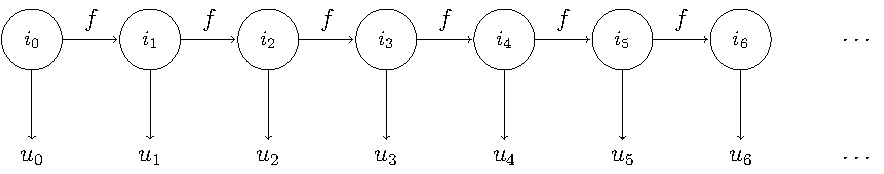
\includegraphics[width=\textwidth]{DCMT_rng.pdf}
  \caption[width=.6\textwidth]{\label{fig:rng1} \it\footnotesize
    \textbf{Random Number Generator.} A RNG is an algorithm
    that produces a sequence
    of floating numbers, says $u_0, u_1, \ldots$, that resembles a
    sequence of independant random numbers, uniformly distributed over
    $[0;1)$.
    It uses a sequence of
    internal states, say $i_0, i_1,\ldots$, which are computed by
    reccurence, namely, $i_{k+1}=f(i_k)$. The first internal state
    $i_0$ is often named the seed.}
\end{minipage}
\end{figure}

The second
version of DIYABC uses the Dynamic Creator (DCMT) of
\citet{DCMT} to look for a set of independent
Mersenne-Twister generators. Actually, the updating function $f$ of a
Mersenne-Twister generator is parametrized by a few integer
numbers. 
The output of the DCMT is a set of $N$ updating functions,
say $\{f^{(1)}, \ldots, f^{(N)}\}$, producing independent streams. 
That is, the $n$-th RNG is a sequence of iternal states
$i_0^{(n)},i_1^{(n)}, i_2^{(n)}, \ldots$ satisfying
$i_{k+1}^{(n)}=f^{(n)}(i_k^{(n)})$
that gives rise to a sequence of independent, uniformly distributed numbers
$u_0^{(n)}, u_1^{(n)}, u_2^{(n)},\ldots$.
We found that the DCMT was simple to use and gave good results.  There
is no limitation on the number $N$ of RNGs it produces. Once initialized,
the different RNGs do not require any communication between them and
each of them runs as quickly as a single Mersenne-Twister
generator. But an important limitation is that it is impossible to add a
new RNG to the set produced by the DCMT. Practically, this means that
we have to know \textit{a priori} a bound on the number of
jobs working together in parallel. See XXX Alex XXX.





%%% Local Variables: 
%%% mode: latex
%%% TeX-master: "Notice_DIYABC_principal"
%%% End: 



  

%%% Local Variables: 
%%% mode: latex
%%% TeX-master: "compilateur"
%%% End: 
